\documentclass{beamer}

\usepackage[utf8x]{inputenc}
\usepackage[english,serbian]{babel}
\usepackage{pgfplots}
\usepackage{listings}
\pgfplotsset{compat=1.10}
\usetikzlibrary{calc} 

\definecolor{RYB1}{RGB}{128, 177, 211}
\definecolor{RYB2}{RGB}{251, 128, 114}
\definecolor{RYB3}{RGB}{253, 180, 98}

\lstdefinelanguage{Swift}{
  keywords={associatedtype, class, deinit, enum, extension, func, import, init, inout, internal, let, operator, private, protocol, public, static, struct, subscript, typealias, var, break, case, continue, default, defer, do, else, fallthrough, for, guard, if, in, repeat, return, switch, where, while, as, catch, dynamicType, false, is, nil, rethrows, super, self, Self, throw, throws, true, try, associativity, convenience, dynamic, didSet, final, get, infix, indirect, lazy, left, mutating, none, nonmutating, optional, override, postfix, precedence, prefix, Protocol, required, right, set, Type, unowned, weak, willSet},
  ndkeywords={class, export, boolean, throw, implements, import, this},
  sensitive=false,
  comment=[l]{//},
  morecomment=[s]{/*}{*/},
  morestring=[b]',
  morestring=[b]"
}

\newcommand\todos[1]{\textcolor{red}{#1}}

\newtheorem{primer}{Primer}[section]

\definecolor{mygreen}{rgb}{0,0.6,0}
\definecolor{mygray}{rgb}{0.5,0.5,0.5}
\definecolor{mymauve}{rgb}{0.58,0,0.82}

\lstset{ 
  backgroundcolor=\color{white},   % choose the background color; you must add \usepackage{color} or \usepackage{xcolor}; should come as last argument
  basicstyle=\footnotesize,        % the size of the fonts that are used for the code
  breakatwhitespace=false,         % sets if automatic breaks should only happen at whitespace
  breaklines=true,                 % sets automatic line breaking
  captionpos=b,                    % sets the caption-position to bottom
  commentstyle=\color{blue},    % comment style
  deletekeywords={...},            % if you want to delete keywords from the given language
  escapeinside={\%*}{*)},          % if you want to add LaTeX within your code
  extendedchars=true,              % lets you use non-ASCII characters; for 8-bits encodings only, does not work with UTF-8
  firstnumber=1000,                % start line enumeration with line 1000
  frame=single,	                   % adds a frame around the code
  keepspaces=true,                 % keeps spaces in text, useful for keeping indentation of code (possibly needs columns=flexible)
  keywordstyle=\color{mygreen},       % keyword style
  language=Swift,                 % the language of the code
  morekeywords={*,...},            % if you want to add more keywords to the set
  numbers=left,                    % where to put the line-numbers; possible values are (none, left, right)
  numbersep=5pt,                   % how far the line-numbers are from the code
  numberstyle=\tiny\color{mygray}, % the style that is used for the line-numbers
  rulecolor=\color{black},         % if not set, the frame-color may be changed on line-breaks within not-black text (e.g. comments (green here))
  showspaces=false,                % show spaces everywhere adding particular underscores; it overrides 'showstringspaces'
  showstringspaces=false,          % underline spaces within strings only
  showtabs=false,                  % show tabs within strings adding particular underscores
  stepnumber=2,                    % the step between two line-numbers. If it's 1, each line will be numbered
  stringstyle=\color{mymauve},     % string literal style
  tabsize=2,	                   % sets default tabsize to 2 spaces
  title=\lstname                   % show the filename of files included with \lstinputlisting; also try caption instead of title
}

\mode<presentation> {

\usetheme{PaloAlto}
}

\usepackage{graphicx} % Allows including images
\usepackage{booktabs} % Allows the use of \toprule, \midrule and \bottomrule in tables

%----------------------------------------------------------------------------------------
%	TITLE PAGE
%----------------------------------------------------------------------------------------

\title[]{Razvoj i primena programskog jezika Swift} % The short title appears at the bottom of every slide, the full title is only on the title page

\author[]{Anđelković Dragica, Mandić Igor, Nikolić Igor, Pejović  Petar} % Your name
\institute[Matf] % Your institution as it will appear on the bottom of every slide, may be shorthand to save space
{
Matematički fakultet \\ % Your institution for the title page
\medskip
\textit{andjelkovic.dragica96@gmail.com, igormandic996@gmail.com, \\ igor.nikolic032@hotmail.com, petar.pejovic8@gmail.com} % Your email address
}
\date{\today} % Date, can be changed to a custom date

\begin{document}

\begin{frame}
\titlepage % Print the title page as the first slide
\end{frame}

\begin{frame}
\frametitle{Uvod} % Table of contents slide, comment this block out to remove it
\tableofcontents % Throughout your presentation, if you choose to use \section{} and \subsection{} commands, these will automatically be printed on this slide as an overview of your presentation

\end{frame}

%----------------------------------------------------------------------------------------
%	PRESENTATION SLIDES
%----------------------------------------------------------------------------------------

%------------------------------------------------
\section{Nastanak i istorijski razvoj}
%------------------------------------------------
\begin{frame}
\frametitle{Nastanak i istorijski razvoj}

\begin{itemize}
\item  Razvoj je započeo 2010. godine Chris Lattner \cite{mastering_swift3}.
\item  Predstavljen je na međunarodnoj konferenciji programera 2014. godine, uz  Xcode 6 \cite{thenextweb_sajt}.
\item Apple je zvanično objavio Swift u decembru 2015. godine, kao projekat otvorenog k\^{o}da i pokrenuo je veb sajt.
\item Do danas je izbačeno 5 verzija Swift-a:
\begin{itemize}
\item{Swift 1.0} - 2014. godine
\item{Swift 2.0} - 2015. godine
\item{Swift 3.0} - 2016. godine
\item{Swift 4.0} - 2017. godine
\item{Swift 5.0} - 2019. godine
\end{itemize}
\end{itemize}
\end{frame}

%------------------------------------------------
\subsection{Mesto u razvojnom stablu}
%------------------------------------------------
\begin{frame}
\frametitle{ Mesto u razvojnom stablu}

\begin{figure}[h!]
\begin{center}
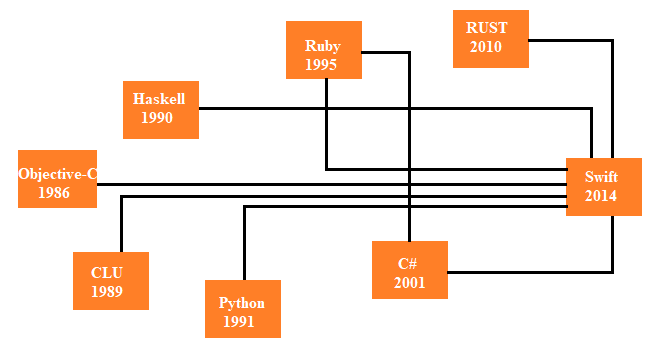
\includegraphics[scale=0.5]{razvojno_stablo.png}
\end{center}
\caption{Razvojno stablo}
\label{fig:razvojno_stablo}
\end{figure}
\end{frame}

%------------------------------------------------
\subsection{Uticaji drugih programskih jezika}
%------------------------------------------------
\begin{frame}
\frametitle{Uticaji drugih programskih jezika}

\begin{table}[h!]
\begin{center}
\caption{Preuzeti koncepti iz drugih programskih jezika}
\begin{tabular}{|l|l|} \hline
\label{tab:koncepti}
\textbf{Programski jezik} & \textbf{Preuzeti koncepti} \\ \hline
JavaScript & Struktura podataka - rečnik  \\ \hline
Scala i Opa & Zaključivanje tipova \\ \hline
Cold Fusion i JSP & Interpolacija Stringa \\ \hline
Python & Opciono naznačavanje kraja naredbe \\ \hline
Java i C\# & Protokoli (Interfejsi) \\ \hline
Lisp i Python & Torke (eng.~{\em Tuples}) \\ \hline
Lisp i JavaScript &  Closure funkcije \\ \hline
C\# i Objective-C & Označeni i neoznačeni celi brojevi \\ \hline
\end{tabular}
\end{center}
\end{table}
\end{frame}

%------------------------------------------------
\section{Osnovna namena, svrha i mogućnosti}
%------------------------------------------------
\begin{frame}
\frametitle{Osnovna namena, svrha i mogućnosti}

\begin{columns}[t]
\column{.5\textwidth}
Osnovna namena:
\begin{itemize}
\item iOS i macOS aplikacije
\item Aplikacije za iPhone i iPad uređaje
\item Server aplikacije
\item Razvoj IoT aplikacija
\item Za Linux operativni sistem
\item Radi se na
stvaranju Swift aplikacija koje će se izvršavati i na Android platformama
\end{itemize}

\column{.5\textwidth} 
Neke od mogućnosti koje pruža su \cite{mastering_swift3}:
\begin{itemize}
\item{Automatsko utvrđivanje tipova}
\item{Sintaksa zatvorenog izraza}
\item{Generički tipovi}
\item{Pseudoklase}
\item{Višestruki povratni tipovi}
\item{Preklapanje operatora}
\end{itemize}
Funkcija Xcode-a \textbf{Mix and match}.

\end{columns}
\end{frame}
%------------------------------------------------
\section{Osnovne osobine}
%------------------------------------------------
\begin{frame}
\frametitle{Osnovne osobine}

\begin{columns}[t]
\column{.5\textwidth} 
Osnovne osobine \cite{swift_programming}:
\begin{itemize}
\item{\textbf{Objektno orijentisan}}
\item{\textbf{Funkcionalan}}
\item{\textbf{Jasan}}
\item{\textbf{Bezbedan}}
\item{\textbf{Ekonomičan}}
\item{\textbf{Upravlja memorijom}}
\item{\textbf{Kompatibilnost sa razvojnim okruženjem Cocoa}}
\end{itemize}

\column{.5\textwidth} 
Podržane paradigme:
\begin{itemize}
\item{\textbf{Objektno orijentisana paradigma}}
\item{\textbf{Funkcionalana paradigma}}
\item{\textbf{Imperativna paradigma}}
\end{itemize}

\end{columns}
\end{frame}

%------------------------------------------------

%------------------------------------------------
\begin{frame}
\frametitle{Osnovne osobine}

\begin{figure}[hbt!]
\begin{tikzpicture}
\pgfplotsset{width=10 cm, height = 5cm}
\begin{axis} [
symbolic x coords={Swift, Python, Ruby, C++, Java, JavaScript, C, SQL, PHP},
xtick={Swift, Python, Ruby, C++, Java, JavaScript, C, SQL, PHP},
x tick label style={rotate=45, anchor=east, align=center},
axis lines*=left,
ymajorgrids = true,
ylabel=Zarada u hiljadama,
legend style={at={(0.5,-0.10)},
    anchor=north,legend columns=1},
    ymin=80,
    ytick={80,90,...,120},
    ymax=120,
    bar width=5mm,
    ybar=-0.5cm, 
   enlarge x limits={abs=0.6cm},
    nodes near coords,        
    every node near coord/.append style={color=black},
]
\addplot [RYB3,fill=RYB3]
coordinates{ (Swift,115) } ;
\addplot [RYB2,fill=RYB2]
coordinates{ (Python,107) } ;
\addplot [RYB1,fill=RYB1]
coordinates{ (Ruby,107)  } ;
\addplot [RYB2,fill=RYB2]
coordinates{ (C++,104) } ;
\addplot [RYB2,fill=RYB2]
coordinates{ (Java,102) } ;
\addplot [RYB1,fill=RYB1]
coordinates{ (JavaScript,99) } ;
\addplot [RYB3,fill=RYB3]
coordinates{ (C,94)  } ;
\addplot [RYB1,fill=RYB1]
coordinates{ (SQL,92) } ;
\addplot [RYB3,fill=RYB3]
coordinates{ (PHP,89)  } ;

\end{axis}

\end{tikzpicture}
\caption{Najplaćeniji programski jezici u Americi 2016. godine}
\label{fig:grafikon}
\end{figure}
\end{frame}

%------------------------------------------------
\section{Okruženja}
%------------------------------------------------
\begin{frame}
\frametitle{Okruženja i njihove karakteristike}

Programski jezik Swift je podržan od strane različitih okruženja, među kojima su najpoznatija:

\begin{itemize}
\item \textbf{Xcode}
\item \textbf{Playground}
\item \textbf{Cocoa Touch}
\item \textbf{SublimeText}
\item \textbf{Atom}
\end{itemize}
\end{frame}
%------------------------------------------------
\section{Instalacija i uputstvo za pokretanje}
%------------------------------------------------
\begin{frame}
\frametitle{Instalacija i uputstvo za pokretanje}

Programski jezik Swift se može koristiti na različitim operativnim sistemima:\\

\begin{itemize}

\item{\textbf{Windows operativni sistem:}}
\begin{itemize}
\item{Preuzimanje sa oficijalnog sajta}
\item{Instalacija Swift-a i kompajlera za Swift}
\item{Izvorni k\^{o}d programa ima ekstenziju \underline{.swift}}
\item{Za kompajliranje i pokretanje primenjuje se korisnički interfejs Swift-a}
\end{itemize}

\item{\textbf{MAC operativni sistem:}}
\begin{itemize}
\item{Dovoljno je preuzeti i instalirati Xcode razvojno okruženje}
\end{itemize}

\end{itemize}
\end{frame}

%------------------------------------------------

%------------------------------------------------
\begin{frame}[fragile]
\frametitle{Instalacija i uputstvo za pokretanje}

\begin{itemize}
\item \textbf{Linux operativni sistem:}
\begin{lstlisting}[language=bash, caption={Instaliranje Swift-a}]
wget https://swift.org/builds/ubuntu1510/swift-2.2-SNAPSHOT-2015-12-10-a/swift-2.2-SNAPSHOT-2015-12-10-a-ubuntu15.10.tar.gz
	
tar -xvzf swift-2.2-SNAPSHOT*
cd swift-2.2-SNAPSHOT*
cd usr/bin
pwd
export PATH=path_to_swift_usr_bin:$PATH
sudo apt-get install clang libicu-dev
swift -version
swift imeprograma.swift
./imeprograma
\end{lstlisting}
\end{itemize}

\end{frame}

%------------------------------------------------
\section{Primeri}
%------------------------------------------------
\begin{frame}[fragile]
\frametitle{Primeri}

\begin{lstlisting}[language=Swift, caption={Ispis teksta},frame=single, label=simple]
print("Hello world!")				    // Hello World!
print("Hello world!");					// Hello World!
\end{lstlisting}

\begin{lstlisting}[language=Swift, caption={Stringovi i konkatenacija stringova},frame=single, label=simple]
var ime = "Swift"
var jezik = "programski jezik"

var poruka = " je najbolji "
var poruka1 = "\ (ime) je najbolji \ (jezik) !" 

print(ime,poruka,jezik,"!")
// Swift je najbolji progmski jezik!
print(poruka1) 
// Swift je najbolji progmski jezik!
\end{lstlisting}

\end{frame}

%------------------------------------------------

%------------------------------------------------
\begin{frame}[fragile]
\frametitle{Primeri}

\begin{lstlisting}[language=Swift, caption={Klasa},frame=single, label=simple]
class Osoba {
    var ime: String
    var godine: Int
    
    init(ime: String, godine: Int) {
        self.ime = ime
        self.godine = godine
    }
    func getIme() -> String {
        return "Tvoje ime je \(self.ime)"
	}
}
var osoba1 = Osoba(ime: "Daca", godine: 22)
print(osoba1.getIme))								// Daca
\end{lstlisting}


\end{frame}

%------------------------------------------------
\section{Specifičnosti}
%------------------------------------------------
\begin{frame}
\frametitle{Specifičnosti}

Swift se dobro štiti od najzastupljenih programskih grešaka usvajanjem modernih paterna programiranja \cite{swift_sajt}:
\begin{itemize}
\item Promenljive su uvek inicijalizovane pre upotrebe
\item Obrađena je greška za pristupanje nepostojećem elementu niza (eng.~{\em out of bounds})
\item Celi brojevi (eng.~{\em integers}) su provereni za prekoračenje memorije (eng.~{\em overflow})
\item Opcione promenljive zahtevaju eksplicitno rukovanje
\item Memorijom se upravlja automatski
\item Rukovanje greškama omogućava kontrolisani oporavak od neočekivanih prekida (eng.~{\em crash})
\end{itemize}

\end{frame}

%------------------------------------------------
\section{Literatura}
%------------------------------------------------

\begin{frame}
\frametitle{Literatura}

\bibliographystyle{plain}
\bibliography{seminarski}
\end{frame}
\end{document} 